\chapter{LIMITATIONS OF A THREE-WIRE DVR IN DISTRIBUTION SYSTEM}

In previous chapters, it is discussed that the dynamic voltage restorer (DVR) is connected to the distribution feeder through the single-phase injection transformers. The primaries of the transformers can be connected in three configurations such as delta, star with isolated neutral and star with neutral connected to filter capacitors neutral point, as shown in Fig.\,\ref{B1.fig2}. This appendix focuses on evaluating the performance of a three-wire DVR using these three transformer configurations. 
\begin{figure*}[]\centering
	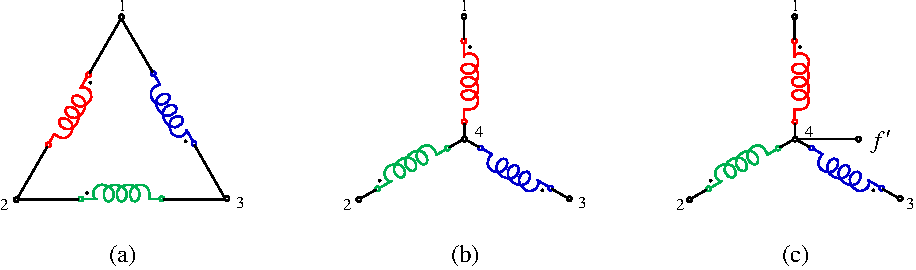
\includegraphics[scale=0.75]{figures/Appendix/TF_Config.pdf}
	\caption{Transformer primary winding configurations: (a) Delta, (b) Star with isolated neutral and (c) Star with neutral connected to filter capacitors neutral} %\vspace*{-0.4cm}
	\label{B1.fig2}
\end{figure*} 

The delta configuration is widely recognized for enabling the flow of zero sequence current but does not facilitate zero sequence voltage injection. Consequently, this configuration adversely affects the DVR's ability to compensate and regulate load voltage during unbalanced voltage sag/swell situations that involve zero sequence voltage components. On the other hand, the two star configurations allow for zero sequence voltage injection. However, the star configuration with an isolated neutral does not provide a path for zero sequence current flow. As a result, the DVR fails to regulate load voltage for unbalanced loads, regardless of the type of voltage disturbance. In the case of the other star configuration, although it allows for the flow of zero sequence current, the presence of filter capacitors prevents this current flow due to their low impedance specifically designed for switching frequency components. This causes the DVR to also fail in regulating load voltage for unbalanced loads with this particular configuration. To verify these conclusive statements, simulation results obtained from MATLAB-Simulink are utilized. 

\begin{figure*}[]\centering
	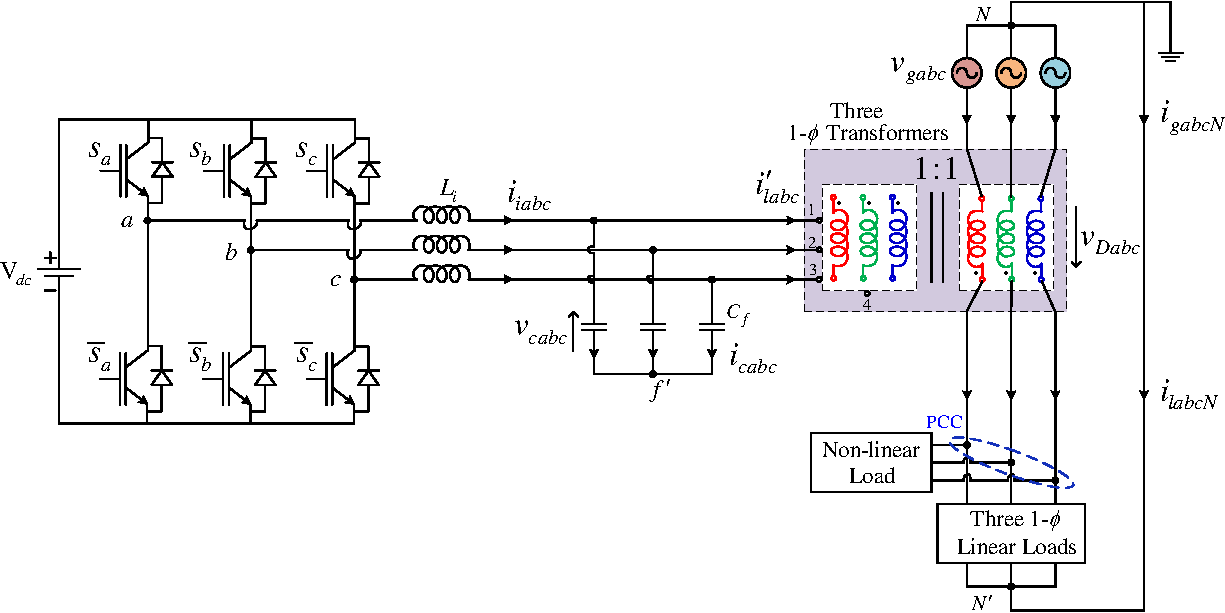
\includegraphics[scale=0.72	]{figures/Appendix/3leg_DVR.pdf}
	\caption{Schematic diagram of three-leg voltage source converter based DVR} %\vspace*{-0.4cm}
	\label{B1.fig1}
\end{figure*} 


The proposed control scheme in Chapter \ref{5.Chap:DVR} is extended to the three-wire DVR connected in a distribution system as shown in Fig.\,\ref{B1.fig1}. The system parameters considered for the simulation study are listed in Table\,\ref{TableB1.2}.
\begin{table}[] 
	\centering
	\caption{System parameters for simulation study}
	\label{TableB1.2}
	\begin{tabular}{>{\small}l>{\small}l}  
		\hline
		\hline
		\textbf{\footnotesize System parameters} & \textbf{\footnotesize Values}\\
		\hline
		\footnotesize Rated supply phase voltage & \footnotesize$230 ~\si{V}, 50 ~\si{Hz}$ \\
		\footnotesize Filter parameters & \footnotesize $L_{i} = 5 ~\si{mH}$, $C_{f} = 30 \, \si{\micro F	}$ \\ 
		\footnotesize DC link voltage & \footnotesize $V_{dc} = 900 ~\si{V}$ \\
		\footnotesize $1-\phi$ Transformer & \footnotesize $50 \, \si{kVA}, 230/230 \, \si{V}, L_{t} = 1.5 \, \si{mH	}$ \\
		\footnotesize Unbalanced linear load  &  \footnotesize $Z_{a} = 1.7+j5.567\,\si{\Omega}$, \\ & \footnotesize $Z_{b} = 50+j58.72\, \si{\Omega}$, \\  & \footnotesize $Z_{c} = 5.25+j15.15\, \si{\Omega}$ \\
		\footnotesize Balanced linear load  &  \footnotesize $Z_{a} = Z_{b} = Z_{c} = 17+j55.67\,\si{\Omega}$ \\ 
		\hline
		\hline 
	\end{tabular} %\vspace*{-0.25cm}
\end{table} 

\begin{sidewaysfigure}[]\centering
	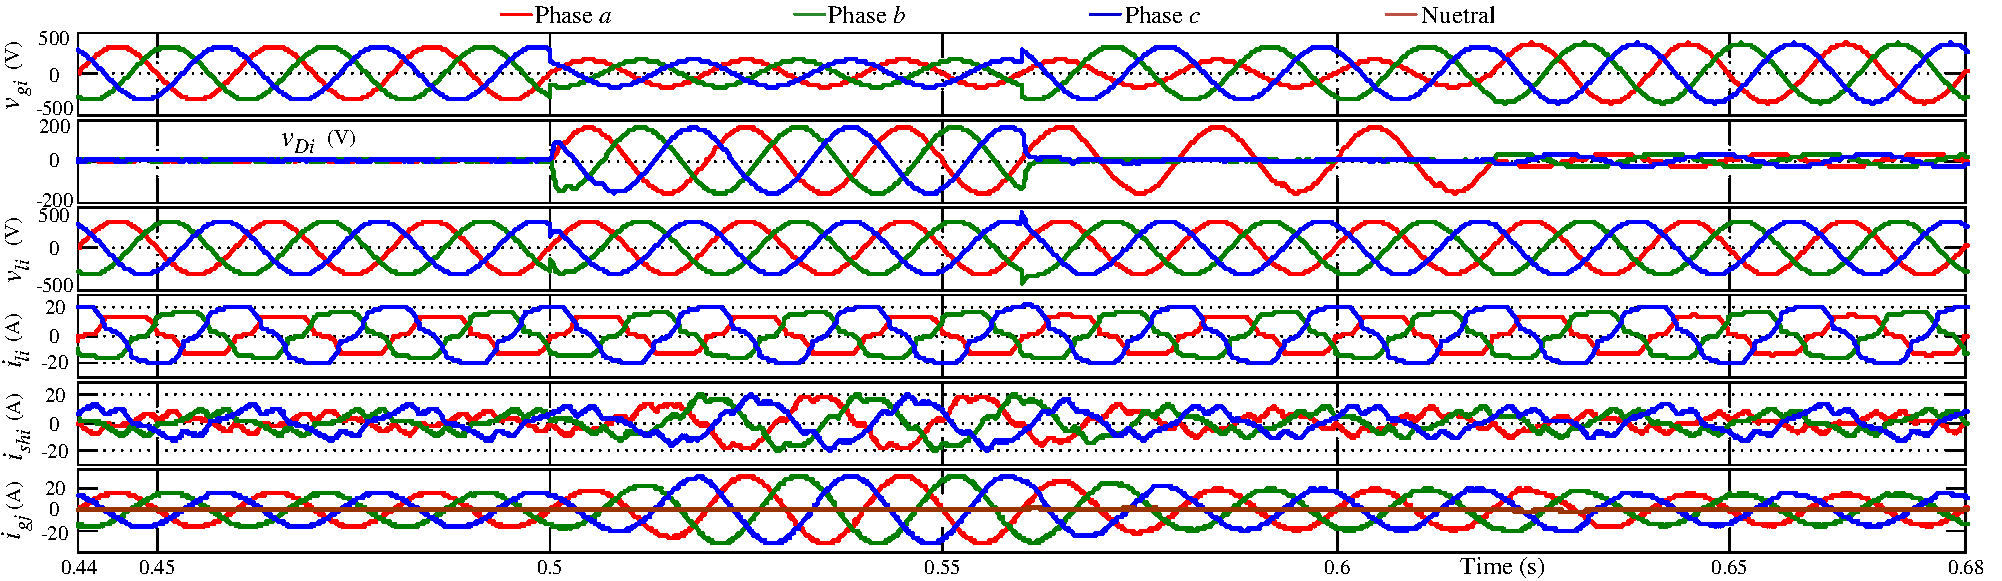
\includegraphics[scale=0.8	]{figures/Appendix/Res1.pdf}
	\caption{Simulation results: (a) Grid voltages and (b) Zero sequence component of grid voltages} %\vspace*{-0.4cm}
	\label{B1.Res1}
	\vspace*{1cm}
	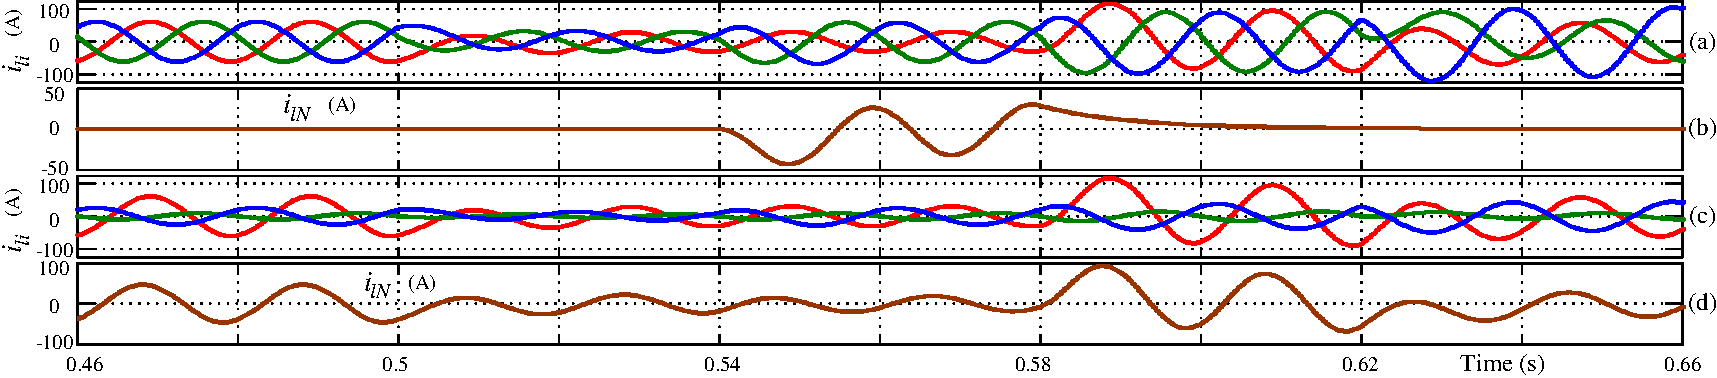
\includegraphics[scale=0.8	]{figures/Appendix/Res2.pdf}
	\caption{Simulation results in the absence of DVR; The load currents ($i_{li}$) and its neutral current ($i_{lN}$): (a) \& (b) Balanced load, and (c) \& (d) Unbalanced load} %\vspace*{-0.4cm}
	\label{B1.Res2}
\end{sidewaysfigure} 
The simulation results include several system parameters, namely grid voltages ($v_{gi}$), load voltages ($v_{li}$), DVR injected voltages ($v_{Di}$), load currents ($i_{li}$), transformer primary currents ($i^\prime_{li}$), and zero sequence components of grid voltages ($v_{g0}$) and load currents ($i_{lN}$). In Fig.\,\ref{B1.Res1}(a), the grid voltage anomalies are presented, including fundamental balanced sag ($v_{gi} = 0.5$ pu), unbalanced sag ($v_{ga} = 0.5$ pu), balanced swell ($v_{gi} = 1.5$ pu), and unbalanced swell with no zero sequence component ($v_{ga} = 1\angle\ang{30}$ pu, $v_{gb} = 1\angle\ang{-30}$ pu, $v_{gc} = \sqrt{3}\angle\ang{180}$ pu). These anomalies occur at specific time instances: $0.5$ s, $0.54$ s, $0.58$ s, and $0.62$ s, respectively. Each voltage anomaly lasts for a duration of $0.04$ s. It is important to note that the same grid voltage profile is utilized for studying the DVR with each transformer configuration. Additionally, Fig.\,\ref{B1.Res1}(b) indicates that the zero sequence component exists in the grid voltage only during the period of unbalanced sag. Furthermore, Fig.\,\ref{B1.Res2} displays the load currents for both balanced and unbalanced loads in the absence of the DVR.

Fig.\,\ref{B1.Res3} illustrates the DVR injected voltages and load voltages for both balanced and unbalanced loads in the case of the delta configuration. It can be observed that, regardless of load unbalance, the DVR effectively regulates the load voltage for all voltage anomalies except during the period of unbalanced sag. This observation provides clear evidence that the DVR with the delta configuration is unable to mitigate unbalanced voltage disturbances with zero sequence components.
 
\begin{sidewaysfigure}[]\centering
	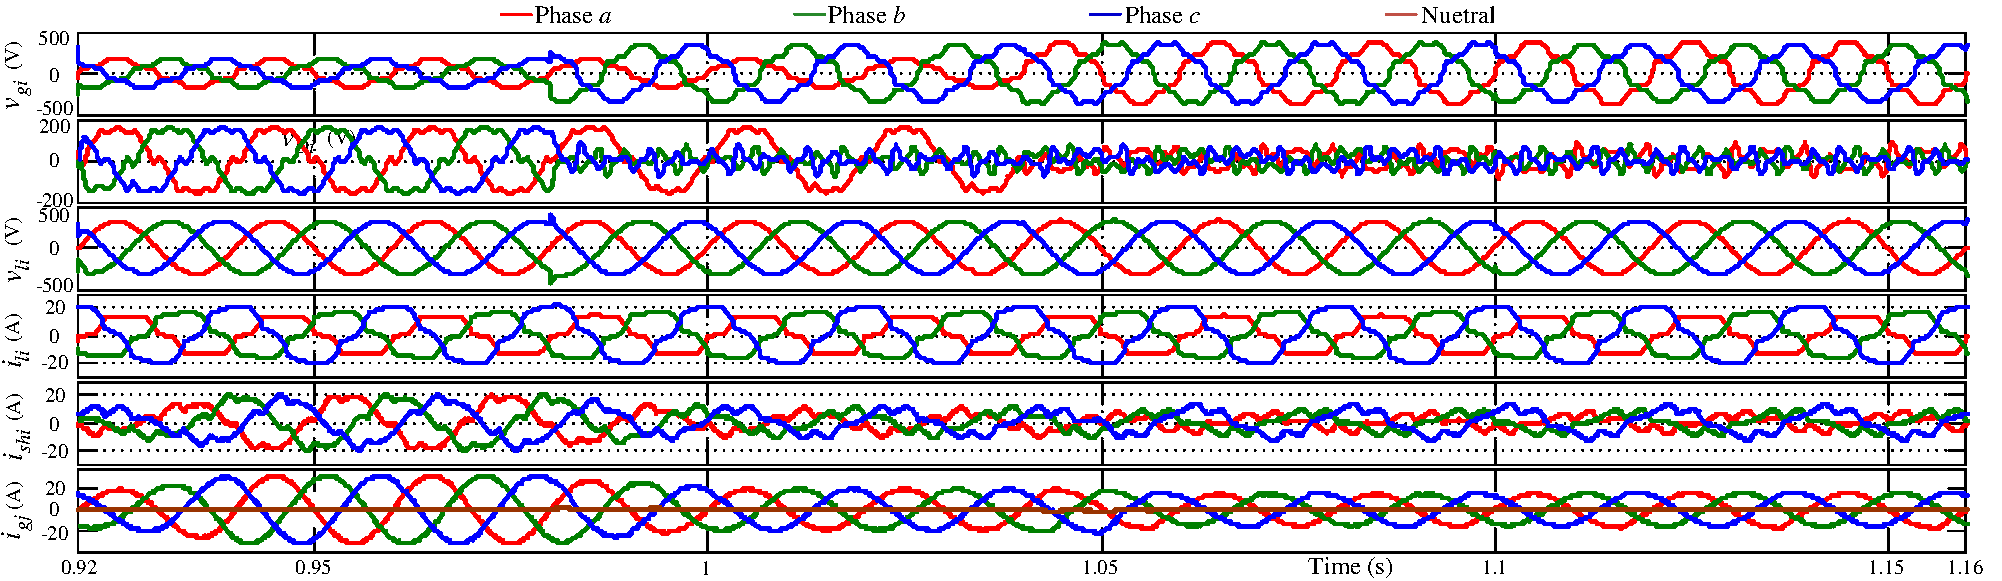
\includegraphics[scale=0.7	]{figures/Appendix/Res3.pdf}
	\caption{Simulation results for a delta configuration; The DVR voltages ($v_{Di}$) and load voltages ($v_{li}$): (a) \& (b) Balanced load, and (c) \& (d) Unbalanced load} %\vspace*{-0.4cm}
	\label{B1.Res3}
	\vspace*{0.5cm}
	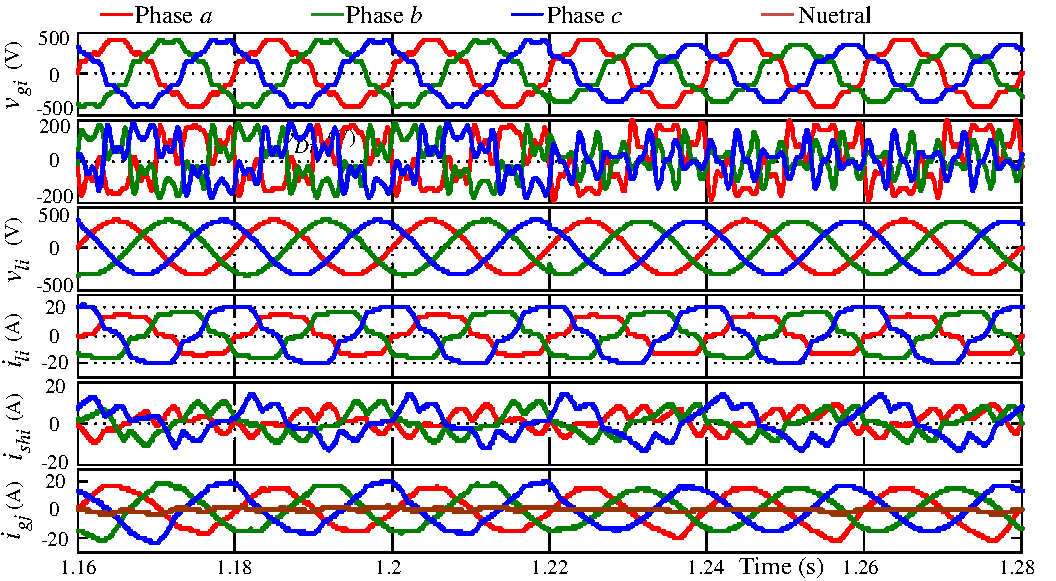
\includegraphics[scale=0.7	]{figures/Appendix/Res4.pdf}
	\caption{Simulation results for a star with isolated neutral configuration; The DVR voltages ($v_{Di}$), load voltages ($v_{li}$) and transformer primary currents ($i^{\prime}_{li}$):  (a), (b) \& (c) Balanced load, and (d), (e) \& (f) Unbalanced load} %\vspace*{-0.4cm}
	\label{B1.Res4}
\end{sidewaysfigure}
\begin{sidewaysfigure}[]\centering
	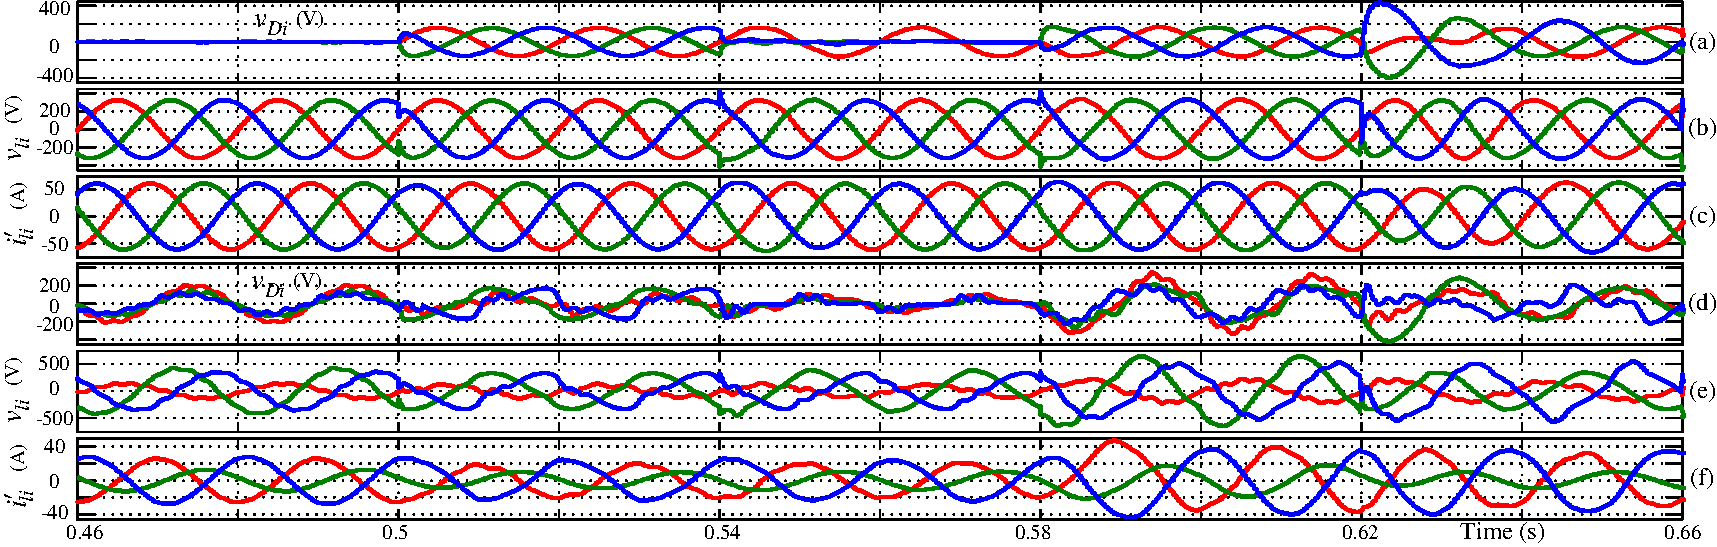
\includegraphics[scale=0.8	]{figures/Appendix/Res5.pdf}
	\caption{Simulation results for a star with neutral connected to filter capacitors neutral configuration; The DVR voltages ($v_{Di}$), load voltages ($v_{li}$) and transformer primary currents ($i^{\prime}_{li}$): (a), (b) \& (c) Balanced load, and (d), (e) \& (f) Unbalanced load} %\vspace*{-0.4cm}
	\label{B1.Res5}
\end{sidewaysfigure}
Fig.\,\ref{B1.Res4}(a)-(c) depict the DVR injected voltages, load voltages, and transformer primary currents for a balanced load in the case of star with isolated neutral configuration. Similarly, Fig.\,\ref{B1.Res4}(d)-(f) represent the same parameters for an unbalanced load. Likewise, in the case of the star configuration with the neutral connected to the filter capacitors, Fig.\,\ref{B1.Res5}(a)-(c) showcase the DVR injected voltages, load voltages, and transformer primary currents for a balanced load, while Fig.\,\ref{B1.Res5}(d)-(f) depict the same for an unbalanced load.

Observing Figs.\,\ref{B1.Res4} and \ref{B1.Res5}, it is evident that the star-configured three-leg DVR effectively mitigates all voltage disturbances for balanced loads. However, for unbalanced loads, voltage disturbances remain unresolved due to the absence of a path for zero sequence currents at the transformer primary side. Notably, the successful regulation of load voltage for unbalanced sag indicates the capability of the three-leg DVR to generate zero-sequence voltage. Consequently, a star-configured transformer and converter that facilitate the flow of zero sequence current emerge as the feasible solution for DVR implementation in the secondary distribution system. 

\begin{sidewaystable}
\centering
\caption{The compensation capability of three-leg DVR with three transformer configurations under various grid conditions}
\label{TableB1.3}
\begin{tabular}{>{\small}c>{\small}c>{\small}c>{\small}c>{\small}c>{\small}c>{\small}c>{\small}c>{\small}c>{\small}c}  
	\hline
	\hline
	\textbf{\footnotesize Load $\rightarrow$} & \multicolumn{4}{c}{\textbf{\footnotesize Balanced load}} & & \multicolumn{4}{c}{\textbf{\footnotesize Unbalanced load}} \\ \cline{2-5} \cline{7-10}
	%\hline
	&   & \textbf{\footnotesize Balanced} & \textbf{\footnotesize Unbalanced} & \textbf{\footnotesize Unbalanced}  & & & \textbf{\footnotesize Balanced} & \textbf{\footnotesize Unbalanced} & \textbf{\footnotesize Unbalanced} \\
	\textbf{\footnotesize Grid voltage $\rightarrow$} & \textbf{\footnotesize Normal} & \textbf{\footnotesize sag/swell} & \textbf{\footnotesize sag/swell} & \textbf{\footnotesize sag/swell}  & & \textbf{\footnotesize Normal} & \textbf{\footnotesize sag/swell} & \textbf{\footnotesize sag/swell} & \textbf{\footnotesize sag/swell} \\
	&   &  & \textbf{\footnotesize with $v_{g0} \neq 0$} & \textbf{\footnotesize with $v_{g0} = 0$}  &  &  &  & \textbf{\footnotesize with $v_{g0} \neq 0$} & \textbf{\footnotesize with $v_{g0} = 0$} \\
	\hline
	\footnotesize 1. Delta & \footnotesize \textcolor{blue}{Yes} & \footnotesize \textcolor{blue}{Yes}  & \footnotesize \textcolor{red}{No} & \footnotesize \textcolor{blue}{Yes} &  & \footnotesize \textcolor{blue}{Yes}  & \footnotesize \textcolor{blue}{Yes} & \footnotesize \textcolor{red}{No} & \footnotesize \textcolor{blue}{Yes} \\ 
	\footnotesize 2. Star with isolated neutral & \footnotesize \textcolor{blue}{Yes} & \footnotesize \textcolor{blue}{Yes} &  \footnotesize \textcolor{blue}{Yes} & \footnotesize \textcolor{blue}{Yes} & & \footnotesize \textcolor{red}{No}  & \footnotesize \textcolor{red}{No} & \footnotesize \textcolor{red}{No} & \footnotesize \textcolor{red}{No} \\  
	\footnotesize 3. Star with neutral connected  & \multirow{2}{*}{\footnotesize \textcolor{blue}{Yes}} & \multirow{2}{*}{\footnotesize \textcolor{blue}{Yes}}  & \multirow{2}{*}{\footnotesize \textcolor{blue}{Yes}} & \multirow{2}{*}{\footnotesize \textcolor{blue}{Yes}} & & \multirow{2}{*}{\footnotesize \textcolor{red}{No}}  & \multirow{2}{*}{\footnotesize \textcolor{red}{No}} & \multirow{2}{*}{\footnotesize \textcolor{red}{No}} & \multirow{2}{*}{\footnotesize \textcolor{red}{No}} \\ 
	\footnotesize to filter capacitors neutral &  &   &  & & &   &  &  &  \\
	\hline
	\hline 
\end{tabular}	
\end{sidewaystable} 

The comprehensive analysis of this study is summarized in Table\,\ref{TableB1.3}. The table presents the performance of the DVR in different transformer configurations and system scenarios, indicating whether the DVR successfully maintains load voltages at the desired value ("Yes") or fails to regulate load voltages ("No"). The table offers a clear overview of the DVR's effectiveness under various conditions, enabling easy evaluation.

It has been verified that the three-wire DVR, regardless of the transformer configuration, is unable to regulate load voltages for all possible grid conditions. Consequently, alternative DVR converter topologies need to be explored to achieve load voltage regulation under all grid conditions. The split-capacitor-based three-leg converter and four-leg converter are potential solutions that can provide both zero-sequence voltage injection and current flow, thereby addressing this limitation.
